\documentclass{article}
\usepackage[preprint,nonatbib]{neurips_2026}
\usepackage[T1]{fontenc}
\usepackage[utf8]{inputenc}
\usepackage{booktabs,amsmath,amssymb,graphicx,microtype}
\usepackage[hidelinks]{hyperref}
\usepackage{xurl}
% Generated by scripts/build_report_tables.py; edit the source aggregates only.
\newcommand{\PrimaryResults}{%
\setlength{\tabcolsep}{5pt}
\begin{tabular}{lrrrr}
\toprule
Condition & Published & Clean & Augmented & $\Delta$ (pp) \\
\midrule
Clean & 84.0071 & 84.3437 & 84.4824 & 0.1387 \\
Case loss, mild & 83.0810 $\pm$ 0.1646 & 83.2890 $\pm$ 0.0821 & 83.8620 $\pm$ 0.0832 & 0.5730 $\pm$ 0.0935 \\
Case loss, medium & 81.5050 $\pm$ 0.1071 & 81.6460 $\pm$ 0.1313 & 82.8992 $\pm$ 0.1601 & 1.2532 $\pm$ 0.0505 \\
Case loss, heavy & 79.2674 $\pm$ 0.2516 & 79.1340 $\pm$ 0.2251 & 81.3246 $\pm$ 0.1641 & 2.1906 $\pm$ 0.0618 \\
Diacritic loss, mild & 83.9539 $\pm$ 0.0294 & 84.2402 $\pm$ 0.0265 & 84.4018 $\pm$ 0.0362 & 0.1617 $\pm$ 0.0521 \\
Diacritic loss, medium & 83.8259 $\pm$ 0.0420 & 84.1244 $\pm$ 0.0272 & 84.3583 $\pm$ 0.0273 & 0.2339 $\pm$ 0.0120 \\
Diacritic loss, heavy & 83.6073 $\pm$ 0.0365 & 84.0130 $\pm$ 0.0574 & 84.3013 $\pm$ 0.0579 & 0.2883 $\pm$ 0.1080 \\
Interior swap, mild & 83.6547 $\pm$ 0.0511 & 83.9855 $\pm$ 0.0521 & 84.3291 $\pm$ 0.0368 & 0.3436 $\pm$ 0.0371 \\
Interior swap, medium & 83.1434 $\pm$ 0.0503 & 83.4238 $\pm$ 0.0302 & 84.0301 $\pm$ 0.0204 & 0.6063 $\pm$ 0.0351 \\
Interior swap, heavy & 82.2406 $\pm$ 0.0339 & 82.4574 $\pm$ 0.1407 & 83.5796 $\pm$ 0.1157 & 1.1222 $\pm$ 0.1699 \\
Combined, mild & 82.6204 $\pm$ 0.1460 & 82.8196 $\pm$ 0.0709 & 83.6413 $\pm$ 0.0973 & 0.8217 $\pm$ 0.1358 \\
Combined, medium & 80.4421 $\pm$ 0.0866 & 80.4467 $\pm$ 0.0665 & 82.4459 $\pm$ 0.0919 & 1.9992 $\pm$ 0.0339 \\
Combined, heavy & 77.2021 $\pm$ 0.1631 & 76.7502 $\pm$ 0.3021 & 80.5289 $\pm$ 0.0906 & 3.7787 $\pm$ 0.2191 \\
Full case loss & 77.5536 & 77.3370 & 80.2493 & 2.9123 \\
Full diacritic loss & 82.8649 & 83.5346 & 83.7425 & 0.2079 \\
\bottomrule
\end{tabular}
}
\newcommand{\SensitivityResults}{%
\setlength{\tabcolsep}{5pt}
\begin{tabular}{lrrrr}
\toprule
Condition & Published & Clean & Augmented & $\Delta$ (pp) \\
\midrule
Clean & 83.9760 & 84.2972 & 84.4389 & 0.1417 \\
Case loss, mild & 83.0435 $\pm$ 0.1675 & 83.2359 $\pm$ 0.0830 & 83.8135 $\pm$ 0.0839 & 0.5776 $\pm$ 0.0941 \\
Case loss, medium & 81.4581 $\pm$ 0.1090 & 81.5810 $\pm$ 0.1341 & 82.8438 $\pm$ 0.1628 & 1.2628 $\pm$ 0.0513 \\
Case loss, heavy & 79.2066 $\pm$ 0.2552 & 79.0525 $\pm$ 0.2281 & 81.2574 $\pm$ 0.1674 & 2.2049 $\pm$ 0.0615 \\
Diacritic loss, mild & 83.9227 $\pm$ 0.0298 & 84.1933 $\pm$ 0.0266 & 84.3576 $\pm$ 0.0365 & 0.1643 $\pm$ 0.0526 \\
Diacritic loss, medium & 83.7959 $\pm$ 0.0422 & 84.0771 $\pm$ 0.0272 & 84.3137 $\pm$ 0.0276 & 0.2366 $\pm$ 0.0123 \\
Diacritic loss, heavy & 83.5764 $\pm$ 0.0372 & 83.9659 $\pm$ 0.0590 & 84.2565 $\pm$ 0.0586 & 0.2906 $\pm$ 0.1101 \\
Interior swap, mild & 83.6204 $\pm$ 0.0512 & 83.9366 $\pm$ 0.0536 & 84.2849 $\pm$ 0.0372 & 0.3483 $\pm$ 0.0387 \\
Interior swap, medium & 83.1064 $\pm$ 0.0494 & 83.3725 $\pm$ 0.0312 & 83.9843 $\pm$ 0.0204 & 0.6117 $\pm$ 0.0365 \\
Interior swap, heavy & 82.2034 $\pm$ 0.0340 & 82.4017 $\pm$ 0.1437 & 83.5321 $\pm$ 0.1179 & 1.1304 $\pm$ 0.1711 \\
Combined, mild & 82.5791 $\pm$ 0.1469 & 82.7653 $\pm$ 0.0711 & 83.5917 $\pm$ 0.0992 & 0.8264 $\pm$ 0.1351 \\
Combined, medium & 80.3899 $\pm$ 0.0892 & 80.3793 $\pm$ 0.0707 & 82.3892 $\pm$ 0.0932 & 2.0099 $\pm$ 0.0299 \\
Combined, heavy & 77.1358 $\pm$ 0.1730 & 76.6662 $\pm$ 0.3035 & 80.4613 $\pm$ 0.0919 & 3.7951 $\pm$ 0.2178 \\
Full case loss & 77.4783 & 77.2415 & 80.1728 & 2.9313 \\
Full diacritic loss & 82.8310 & 83.4868 & 83.6958 & 0.2090 \\
\bottomrule
\end{tabular}
}
\newcommand{\AblationResults}{%
\setlength{\tabcolsep}{5pt}
\begin{tabular}{lrrr}
\toprule
Condition & Augmented & Without case & $\Delta$ (pp) \\
\midrule
Clean & 84.4824 & 84.3919 & 0.0905 \\
Case loss, medium & 83.0763 & 82.1178 & 0.9585 \\
Diacritic loss, medium & 84.3712 & 84.3917 & -0.0205 \\
Interior swap, medium & 84.0256 & 84.1335 & -0.1078 \\
Combined, medium & 82.4929 & 81.6129 & 0.8799 \\
\bottomrule
\end{tabular}
}
\newcommand{\ClassResults}{%
\setlength{\tabcolsep}{5pt}
\begin{tabular}{llrr}
\toprule
Input & Class & Clean F1 & Augmented F1 \\
\midrule
Clean & PERIOD & 96.1451 & 96.1348 \\
Clean & COMMA & 63.9560 & 63.9301 \\
Clean & QUESTION\_MARK & 92.9301 & 93.3824 \\
Combined, heavy & PERIOD & 91.5565 $\pm$ 0.0862 & 92.4131 $\pm$ 0.0553 \\
Combined, heavy & COMMA & 51.6579 $\pm$ 0.1776 & 58.7611 $\pm$ 0.1188 \\
Combined, heavy & QUESTION\_MARK & 87.0362 $\pm$ 0.6847 & 90.4125 $\pm$ 0.2312 \\
\bottomrule
\end{tabular}
}
\newcommand{\DiagnosticResults}{%
\setlength{\tabcolsep}{5pt}
\begin{tabular}{llrrr}
\toprule
Input & Model & Edited & Context & Unedited row \\
\midrule
Case loss, heavy & Clean & 352 & 2270 & 0 \\
Case loss, heavy & Augmented & 169 & 1464 & 0 \\
Combined, heavy & Clean & 1600 & 2447 & 0 \\
Combined, heavy & Augmented & 876 & 1579 & 0 \\
\bottomrule
\end{tabular}
}
\newcommand{\CoverageResults}{%
\setlength{\tabcolsep}{5pt}
\begin{tabular}{lrr}
\toprule
Input (seed586 where stochastic) & Changed words & Coverage \\
\midrule
Combined, mild & 10690 & 5.8903\% \\
Combined, medium & 26012 & 14.3329\% \\
Combined, heavy & 49576 & 27.3169\% \\
Case loss full & 24408 & 13.4490\% \\
Diacritic loss full & 75769 & 41.7495\% \\
\bottomrule
\end{tabular}
}
\newcommand{\TrainingHistory}{%
\setlength{\tabcolsep}{5pt}
\begin{tabular}{rrrrr}
\toprule
Epoch & Updates & Clean & Augmented & Without case \\
\midrule
1 & 3656 & 83.2543 & 83.3313 & 83.1426 \\
2 & 7312 & 83.4822 & 83.3883 & 83.5030 \\
3 & 10968 & \textbf{84.0365} & \textbf{83.9881} & \textbf{84.1310} \\
\bottomrule
\end{tabular}
}

\title{Robustness of Turkish Punctuation Restoration\\under Informal Writing Noise}
\author{Kagan Can\\CMPE 586 Course Project\\
\href{https://github.com/kckagancan/cmpe586-turkish-punctuation}{\texttt{github.com/kckagancan/cmpe586-turkish-punctuation}}
\ifdefined\CourseSubmission\input{private-author.tex}\fi
}
\begin{document}
\maketitle
\begin{abstract}
Punctuation restoration models can depend on orthographic cues that disappear
in informal writing. We study Turkish casing loss, Turkish character folding,
and internal character transpositions using deterministic perturbations that
preserve word positions and punctuation targets. A published punctuation BERT
provides an external reference. The controlled comparison uses clean and
noise-augmented BERTurk models with identical initialization, examples, data
order, optimizer settings, and three-epoch training budgets. A third training
arm removes case loss without redistributing its noise budget. After
validation-based development, we froze a held-out protocol comprising 122
model--condition evaluations. On 14,600 eligible test rows, augmentation changes
clean punctuation macro-F1 from 84.3437\% to 84.4824\% and improves combined-heavy
macro-F1 from 76.7502\% to 80.5289\%, a paired gain of $3.7787\pm0.2191$
percentage points across three corruption seeds. Removing case loss reduces
matched case-loss and combined-medium F1 by 0.9585 and 0.8799 points,
respectively. An exact-input-overlap sensitivity analysis preserves the main
pattern. These descriptive findings support this controlled augmentation recipe;
one training seed, synthetic noise, and unresolved dataset provenance limit
broader conclusions.
\end{abstract}

\section{Introduction}
Punctuation restoration assigns marks to text whose punctuation is absent. It
is often studied in speech transcription, but written inputs can also contain
inconsistent casing, missing Turkish letters, and typing errors. Such edits
retain the intended word sequence while changing surface evidence available to
a cased Transformer. Turkish is a useful setting because locale-sensitive
\texttt{I/\i/\.{I}/i} casing and explicit Turkish character substitutions require
care beyond generic English lowercasing.

We ask three questions: (1) which defined perturbations and doses reduce
punctuation F1 most; (2) whether training augmentation improves robustness while
maintaining useful clean-text performance; and (3) how punctuation classes and
the case-loss training component contribute to the observed differences.
The core comparison holds training initialization and budget fixed, rather than
attributing differences from an independently trained published model to
augmentation. Every planned held-out condition is reported, including small
negative ablation contrasts.

The contribution is a \emph{controlled Turkish writing-noise study}: deterministic
word-level perturbations with exact target preservation, matched clean/augmented
fine-tuning, a case-loss removal arm, and a reproducible held-out analysis with an
overlap sensitivity cohort. We do not claim a new architecture or the first
combination of punctuation restoration and noise augmentation. The project
repository provides source, frozen recipes, aggregate results, and the report;
raw data and weights are retained separately.

\section{Related work and design choices}
Kurt and \c{C}ay\i r~\cite{kurt2023} release Turkish punctuation data and Transformer
checkpoints. We use their pinned CSV release and published BERT as a reference,
while independently specifying our training and evaluation recipes. BERTurk's
cased encoder~\cite{berturk} initializes all controlled arms. Nagy et
al.~\cite{nagy2021} study BERT punctuation restoration and report punctuation
class metrics. We adopt first-subword token classification and emphasize
punctuation-only macro-F1 with explicit treatment of non-punctuation positions.

Noise-aware punctuation/truecasing training has prior work: Sunkara et
al.~\cite{sunkara2020} use ASR hypotheses. Our spelling transformations preserve
every word slot, so their ASR alignment and deletion rules are not imported.
Belinkov and Bisk~\cite{belinkov2018} and Karpukhin et al.~\cite{karpukhin2019}
motivate examining character noise and augmentation, but their translation
findings do not establish expected Turkish punctuation gains. N\'{a}plava et
al.~\cite{naplava2021} motivate separating orthographic aspects; unlike their
natural-error modeling, our doses are synthetic and are not calibrated to
Turkish user-error frequencies.

CheckList~\cite{ribeiro2020} motivates condition-specific behavioral analysis.
We retain the project's perturbation pipeline rather than use its toolkit.
Lee et al.~\cite{lee2022} motivate documenting overlap; our exact-token-list
sensitivity filter is narrower than document-level deduplication. Dodge et
al.~\cite{dodge2020} motivate the explicit distinction between training-seed
variation and the corruption-seed variation measured here.

\section{Data, task, and controlled perturbations}
\subsection{Release, eligibility, and held-out cohorts}
We use the original train/validation/test CSV partitions from the pinned
release.\footnote{Source revision: \path{7ede7a4ba9e51dad085a7f0d9b6c0a9c32622397}.}
Each word is labeled by the
punctuation \emph{after} it: \texttt{O}, \texttt{PERIOD}, \texttt{COMMA}, or
\texttt{QUESTION\_MARK}. A CSV row can contain several sentences and is not
assumed to be a document boundary. The raw files contain 651 empty word slots
with punctuation labels. Rather than delete targets or merge marks, the fixed
\texttt{clean-v1} policy quarantines each affected row in full.

\begin{table}[htbp]
\centering
\caption{Fixed eligibility policy. Quarantined rows remain locally preserved;
the original CSV files are unchanged.}
\label{tab:data}
\begin{tabular}{lrrr}
\toprule
Split & Released rows & Quarantined rows & Eligible rows / words\\
\midrule
Train & 117,431 & 462 & 116,969 / 1,463,897\\
Validation & 14,514 & 61 & 14,453 / 179,164\\
Test (primary) & 14,661 & 61 & 14,600 / 181,485\\
\bottomrule
\end{tabular}
\end{table}

The primary test cohort retains all eligible released test rows, including
within-test duplicates. A second, fixed sensitivity cohort excludes a test row
if its \emph{original entire token list} exactly matches any released train or
validation input. Case-sensitive token-list hashes use no labels, predictions,
normalization, or length cutoff. The union excludes 155 rows: 148 match train,
90 match validation, and 83 match both. Sensitivity therefore contains 14,445
rows and 181,116 words. It filters the same saved predictions; it is not a second
independent test set. Missing document/talk identifiers leave document-level
independence and near-duplicate separation unresolved.

Dataset licensing and the exact derivation/split provenance of these CSVs have
not been established. The model card's license does not establish a dataset
license. We publish aggregate measurements and source hashes, not the corpus,
raw examples, or trained weights. Our filtered scores are not a direct
reproduction of upstream unfiltered benchmark scores.

\subsection{Noise operators and exact budgets}
Each single-family condition changes exactly
$K=\lfloor Np/100\rfloor$ eligible word positions, where $N$ is the number of
original words in the full primary split and $p\in\{2,5,10\}$ denotes mild,
medium, or heavy. The denominator includes words ineligible for that family.
Thus test budgets are 3,629, 9,074, and 18,148 changed words per family. Stable
SHA-256 rankings use original IDs, a split key, and corruption seeds
586/587/588; labels and model outputs do not enter selection. Severity masks
are nested. Insufficient eligibility stops preparation rather than lowering
the dose. The 10\% maximum was chosen from train-only feasibility statistics;
case-loss eligibility was the narrowest pool, about 13.35\% of training words.

\textbf{Case loss} lowercases selected words with Turkish-specific
\texttt{I}$\rightarrow$\texttt{\i} and \texttt{\.{I}}$\rightarrow$\texttt{i}
handling. \textbf{Diacritic loss} applies the explicit case-preserving map
\texttt{\c{c},\u{g},\i,\"o,\c{s},\"u}$\rightarrow$\texttt{c,g,i,o,s,u}
and its uppercase counterpart. This is a Turkish character-folding operator,
not arbitrary Unicode accent removal. \textbf{Interior swap} exchanges one
adjacent unequal pair strictly inside an eligible alphabetic word of length
at least four, preserving its ends. Short words, digits, apostrophes, and
unsupported characters are ineligible. This operator does not model all typos.

\textbf{Combined} reuses the three single-family plans in the fixed order
swap, case loss, then folding. Overlap is audited, and its union coverage exceeds
each component's budget: for seed586, combined-medium changes 14.3329\% of test
words and combined-heavy changes 27.3169\%. It is a co-occurrence stress, not an
equal-budget interaction estimate. Two separate full-loss endpoints transform
every eligible casing or folding word; their test coverages are 13.4490\% and
41.7495\%, respectively. These endpoints are not additional 10\% conditions.

Every perturbation preserves row/word IDs, word order, and original punctuation
targets. Changed text is retokenized. The first subword receives the word's
label; subsequent subwords, special tokens, and padding receive \texttt{-100}.
No missing word or input longer than 512 subwords is silently dropped or
truncated. All 39 held-out input views passed the recorded audits; the maximum
prepared input length was 172, with no missing words or unknown subwords.
Fixed intended targets do not prove semantic invariance for every corrupted
spelling; ambiguity is part of the synthetic task's limitation.

\section{Matched training and evaluation}
\subsection{Models and augmentation}
\textbf{Published} is the released Turkish punctuation BERT, evaluated as
provided.\footnote{Checkpoint revision: \path{dd8b9481ed3b3c05110d7e041ecbeb6a1c23b8b0}.}
Its training history and prior exposure to this test release are not controlled.
\textbf{Clean}, \textbf{Augmented}, and \textbf{Without case loss} use the same
saved BERTurk encoder/fresh four-class-head initialization at training seed 586.
Their training rows and per-epoch row permutations are identical; each row
appears exactly once per epoch.

In Augmented, exactly $\lfloor0.5\times116{,}969\rfloor=58{,}484$ row IDs per
epoch use a combined-medium view, replacing those rows in place. Remaining rows
use their clean view; no extra training examples are appended. Word plans are
first generated over the entire clean training split, then the selected row
views are mixed. Consequently, ``50\% noisy views'' is neither 50\% corrupted
words nor a guarantee of an edit in every selected row. Selected rows with no
effective edit remain selected. Plans refresh once per epoch with distinct
train-specific seeds. Realized mixed-view coverage is recorded in the input
audits.

Without case loss uses the same initialization, row views, shuffle, remaining
word plans, optimizer, and update budget while removing the case-loss operator.
\emph{The omitted budget is not redistributed.} This estimates removal under
the fixed recipe; reduced total corruption prevents an equal-dose claim about
intrinsic component importance.

\subsection{Optimization and checkpoint selection}
All three arms fine-tune all parameters for three epochs / 10,968 optimizer
updates. AdamW uses learning rate $2\times10^{-5}$, weight decay 0.01 except
bias/LayerNorm parameters, betas $(0.9,0.999)$, epsilon $10^{-8}$, and gradient
clipping at 1.0. Per-device batch 8 with four accumulation steps gives nominal
effective batch 32; partial accumulation is flushed at epoch boundaries.
Unweighted cross-entropy includes O and is normalized by valid word targets
across each accumulation window. Dropout is 0.1; the schedule has 10\% linear
warmup followed by linear decay. Training uses FP32/eager attention on a T4.

Checkpoint selection uses highest clean-validation punctuation macro-F1 at
completed epoch ends, choosing the earlier epoch on an exact tie. All arms
selected epoch 3, so selected and final checkpoints coincide. No noisy-validation
or test score selected a checkpoint. The recipe was fixed after validation
development; no hyperparameter search, training-seed search, or early stopping
was performed. Three epochs are the matched compute budget, not evidence of
convergence or an optimal epoch count.

\subsection{Frozen matrix, numerical controls, and metrics}
Validation comprises three main models $\times39=117$ evaluations, plus five
new ablation evaluations paired with 15 existing references. After these
validation results were inspected, the held-out protocol, models, cohort masks,
conditions, and analysis rules were frozen before project test scoring. It is
\emph{validation-informed}, not a blind preregistration before development.

The held-out matrix contains 39 conditions for each main model: one clean
anchor, $4$ families $\times3$ doses $\times3$ corruption seeds, and two full-loss
endpoints. The ablation has clean plus the four medium/seed586 conditions,
matching its frozen validation scope. Total inference is $3\times39+5=122$
model--condition runs; primary and sensitivity reporting yield 244 score sets
from the same predictions. There is no extra inference for sensitivity.

Inference uses the same Tesla T4 numerical policy across models and conditions:
FP32, SDPA with the math backend, TF32 disabled, deterministic algorithms, batch
16, and four CPU threads. A shared clean-length/row-ID ordering fixes batch
membership. This inference policy differs from training's eager attention;
models are compared under the same recorded inference policy. Actual tensors,
runtime/packages, sources, inputs, and eight validation-only readiness probes
were checked before test scoring. All 122 conditions completed, followed by
independent local recomputation of all 244 cohort scores from saved predictions
and original word targets. No training or inference was repeated for analysis.

For punctuation class $c$, $F_{1,c}=2TP_c/(2TP_c+FP_c+FN_c)$, with zero for a
zero denominator. The primary score is
$(F_{1,\mathrm{PERIOD}}+F_{1,\mathrm{COMMA}}+F_{1,\mathrm{QUESTION}})/3$.
O positions remain in false-positive/negative counts and are omitted only from
the punctuation averages. Macro/micro P/R/F1, class supports, and four-class
confusions are also retained. Values below are percentages; differences are
percentage points (pp). Mean $\pm$ sample SD describes the three \emph{corruption}
seeds only. Paired gains are computed per seed before aggregation, so the gain
SD is not the difference between two marginal SDs. No p-values, confidence
intervals, equivalence claims, or training-seed stability claims are made.

\section{Results and analysis}
\subsection{Main held-out comparison}
\begin{table}[t]
\centering\small
\caption{Complete primary held-out matrix, punctuation macro-F1 (\%). Stochastic
conditions are means $\pm$ sample SD over three corruption seeds. Clean and full
endpoints are deterministic. $\Delta$ is the paired Augmented minus Clean gain
in pp. Ablation values are reported separately in Table~\ref{tab:ablation}.}
\label{tab:primary}
\PrimaryResults
\end{table}

Table~\ref{tab:primary} reports every main-model condition. Clean-text macro-F1
is 84.3437\% for Clean and 84.4824\% for Augmented, a small descriptive
$+0.1387$ pp difference. This observation does not establish clean-performance
equivalence across training runs. Augmentation has positive mean gains in all
listed family/dose groups (Figure~\ref{fig:curves}), with the largest at combined-heavy:
$76.7502\%\rightarrow80.5289\%$ ($+3.7787\pm0.2191$ pp).
The clean-trained model loses 7.5935 pp from its own clean anchor there, whereas
Augmented loses 3.9535 pp. Robustness remains imperfect despite the improvement.

At matched 10\% component word doses, Clean F1 is 79.1340\% under case loss,
84.0130\% under folding, and 82.4574\% under swaps. Case loss is the most damaging
\emph{defined single-family condition} here; different eligible word pools and
character changes prevent a universal ranking of noise types. Gains increase
with severity: case-loss gains rise from 0.5730 to 2.1906 pp and swap gains from
0.3436 to 1.1222 pp. The combined curve is not an interaction estimate because
its changed-word union is larger.

\begin{figure}[t]
\centering
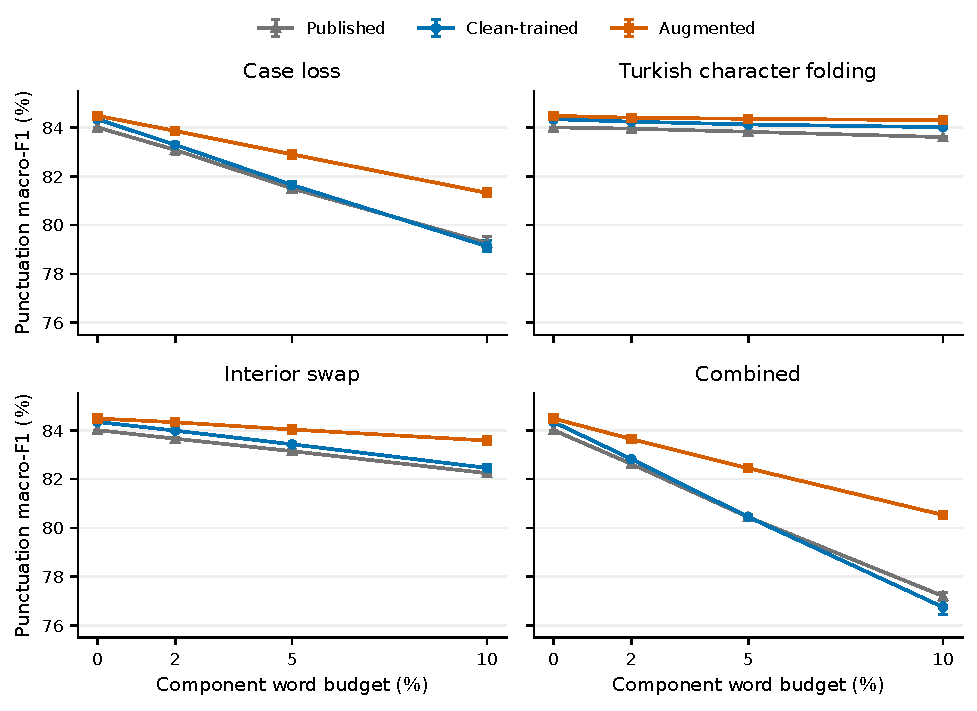
\includegraphics[width=\linewidth]{figures/robustness.pdf}
\caption{Primary held-out severity curves from verified aggregates. Error
bars represent corruption-seed SD, not variation across training runs.
Component doses in the combined panel have a larger union coverage.}
\label{fig:curves}
\end{figure}

Published achieves clean F1 of 84.0071\% and combined-heavy F1 of 77.2021\%.
It slightly exceeds Clean in combined-heavy and some other noisy conditions,
despite lower clean F1. Thus a clean-only ranking hides robustness differences.
This external comparison supplies context; the controlled augmentation estimate
comes from Augmented versus Clean.

\subsection{Class-specific behavior and contextual errors}
\begin{table}[t]
\centering\small
\caption{Primary per-class F1 (\%). Heavy values average three corruption
seeds; clean controls are single deterministic scores.}
\label{tab:classes}
\ClassResults
\end{table}
Commas are the lowest-F1 punctuation class in both clean and combined-heavy text
(Table~\ref{tab:classes}). At combined-heavy, their F1 increases from 51.6579\%
to 58.7611\% with augmentation, a 7.1033 pp gain; period and question-mark gains
are 0.8565 and 3.3763 pp. Equal class weights make these comma errors important
to macro-F1 even though question marks have much smaller support. Clean-test
support is 15,465 periods, 12,164 commas, and 1,228 question marks; O has 152,628
positions. Full class P/R/F1 and confusion matrices remain in the public
aggregate condition file.

The prelisted diagnostics compare each model to its own clean predictions.
At case-loss-heavy/seed586, Clean creates 2,622 new word-class errors, including
2,270 at \emph{unchanged words in edited rows}; Augmented creates 1,633, including
1,464 in that contextual category. At combined-heavy, corresponding totals are
4,047 and 2,455 (Table~\ref{tab:diagnostics}). All entirely unedited rows retain
their clean predictions in these checks. The counts show that edits can affect
predictions beyond the edited word; they do not identify a causal mechanism
inside attention or constitute punctuation-class FP/FN counts. A wrong
punctuation substitution can contribute to more than one class metric.

\subsection{Case-loss training ablation}
\begin{table}[t]
\centering\small
\caption{Matched primary ablation: corruption seed586 only. $\Delta$ is
Augmented minus Without case loss, in pp. Both columns use the same seed;
they must not be compared by subtracting a three-seed main-table mean.}
\label{tab:ablation}
\AblationResults
\end{table}
Retaining case loss improves case-loss-medium F1 by 0.9585 pp and combined-medium
F1 by 0.8799 pp (Table~\ref{tab:ablation}). The clean-test difference is
$+0.0905$ pp. Small differences favor the removal arm under folding
($-0.0205$ pp) and swaps ($-0.1078$ pp). We report these unfavorable contrasts
alongside the positive ones. The ablation's clean-validation advantage
($+0.1430$ pp for removal) does not recur on clean test, illustrating why
validation and held-out roles should remain separate.

\begin{figure}[t]
\centering
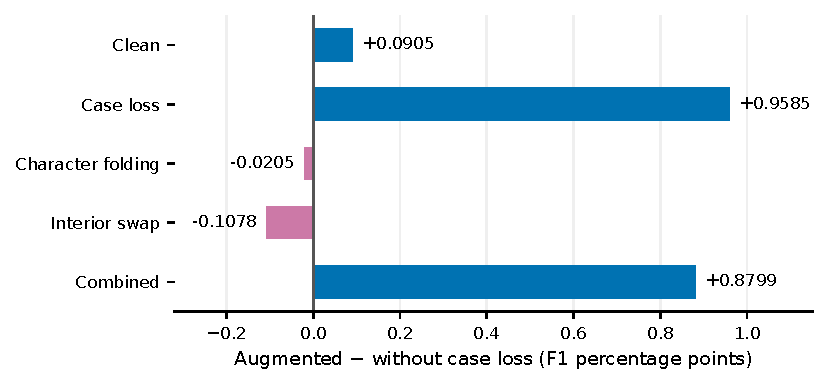
\includegraphics[width=\linewidth]{figures/ablation.pdf}
\caption{Fixed primary-cohort case-loss ablation contrasts.
These are single-corruption-seed, single-training-seed descriptive differences.}
\label{fig:ablation}
\end{figure}
The component is useful against the matching perturbation under this recipe.
Because removal also lowers total training noise, the experiment cannot show
that casing is intrinsically more useful than another component at equal dose.
Only five ablation conditions were planned; no ablation severity sweep or
additional training-seed confirmation was performed.

\subsection{Sensitivity and full-loss endpoints}
Excluding the 155 exact train/validation input matches changes Clean/Augmented
clean F1 to 84.2972\%/84.4389\%. Combined-heavy becomes
76.6662\%/80.4613\%, with a paired gain of $3.7951\pm0.2178$ pp.
Case-loss and combined-medium ablation gains become 0.9637 and 0.8862 pp.
The main descriptive pattern therefore survives this particular overlap filter
(Appendix~\ref{app:sensitivity}); document-level independence remains unverified.

At full case loss, Clean/Augmented F1 is 77.3370\%/80.2493\% ($+2.9123$ pp).
Full folding yields 83.5346\%/83.7425\% ($+0.2079$ pp). These endpoints differ
substantially in coverage and information removed, and cannot be interpreted
as a matched-dose family comparison. Even after augmentation, full casing loss
still reduces performance relative to the clean anchor.

\section{Limitations, responsible use, and conclusion}
There is one training seed and one architecture. Three corruption seeds measure
variation in perturbed inputs, not optimization uncertainty. The three-epoch
budget does not establish convergence or the best achievable clean/robust
trade-off. Synthetic, word-preserving noise omits real deletions, insertions,
phonetic substitutions, broader keyboard errors, and code-switching. Eligibility
and synthetic doses are not estimates of natural Turkish usage. The case-loss
ablation changes both component presence and total noise exposure.

The released CSVs have unresolved licensing and exact split provenance. Exact
input filtering does not remove all near duplicates or establish document
separation; the published model's prior test exposure is unknown. Clean
validation informed the recipe and checkpoint selection. The held-out protocol
was frozen before our test scores, after development; future test-informed
experiments must be identified as exploratory and need new unseen data for
strong independent confirmation. We make no state-of-the-art claim.

Restoration can change the interpretation of questions, boundaries, and pauses.
These experiments do not validate high-stakes deployment or represent all
Turkish speakers' writing. Human review remains appropriate when punctuation
affects meaning. Public artifacts contain aggregate measurements and authored
operator illustrations, while raw text, per-row examples/predictions, and
weights are excluded.

Within these limits, matched noise augmentation improves Turkish punctuation
robustness across the defined perturbation matrix with a small positive clean
F1 difference. The strongest observed benefit is under combined-heavy noise;
case-loss removal weakens matched casing/combined robustness. Class and
contextual diagnostics show where aggregate gains arise and where substantial
errors remain. The result is a reproducible, bounded empirical study rather
than a claim of universal robustness.

\section*{Acknowledgments and tool disclosure}
The project uses the public data/model release by Kurt and \c{C}ay\i r and the
BERTurk encoder. AI assistance (OpenAI Codex) supported implementation,
debugging, literature synthesis, artifact verification, and report preparation.
This disclosure does not assert an independently verified course AI-use policy.
The NeurIPS 2026 preprint style is used for this course report; this document
does not claim NeurIPS submission, acceptance, or peer review.

\clearpage
\begin{thebibliography}{10}
\bibitem{kurt2023} Uygar Kurt and Aykut \c{C}ay\i r. 2023.
Transformer Based Punctuation Restoration for Turkish.
\emph{8th International Conference on Computer Science and Engineering (UBMK)},
169--174. \url{https://doi.org/10.1109/UBMK59864.2023.10286690}.
Release: \url{https://github.com/uygarkurt/Turkish-Punctuation-Restoration}.
\bibitem{berturk} Stefan Schweter. 2020. BERTurk: BERT models for Turkish.
\url{https://github.com/stefan-it/turkish-bert}.
\bibitem{nagy2021} Attila Nagy, Bence Bial, and Judit \'{A}cs. 2021.
Automatic punctuation restoration with BERT models. arXiv:2101.07343.
\url{https://arxiv.org/abs/2101.07343}.
\bibitem{sunkara2020} Monica Sunkara, Srikanth Ronanki, Kalpit Dixit, Sravan
Bodapati, and Katrin Kirchhoff. 2020. Robust Prediction of Punctuation and
Truecasing for Medical ASR. \emph{NLP for Medical Conversations}, 53--62.
\url{https://aclanthology.org/2020.nlpmc-1.8/}.
\bibitem{belinkov2018} Yonatan Belinkov and Yonatan Bisk. 2018. Synthetic and
Natural Noise Both Break Neural Machine Translation. \emph{ICLR}.
\url{https://arxiv.org/abs/1711.02173}.
\bibitem{karpukhin2019} Vladimir Karpukhin, Omer Levy, Jacob Eisenstein, and
Marjan Ghazvininejad. 2019. Training on Synthetic Noise Improves Robustness to
Natural Noise in Machine Translation. \emph{W-NUT}, 42--47.
\url{https://aclanthology.org/D19-5506/}.
\bibitem{naplava2021} Jakub N\'{a}plava, Martin Popel, Milan Straka, and Jana
Strakov\'{a}. 2021. Understanding Model Robustness to User-generated Noisy Texts.
\emph{W-NUT}, 340--350. \url{https://aclanthology.org/2021.wnut-1.38/}.
\bibitem{ribeiro2020} Marco Tulio Ribeiro, Tongshuang Wu, Carlos Guestrin, and
Sameer Singh. 2020. Beyond Accuracy: Behavioral Testing of NLP Models with
CheckList. \emph{ACL}, 4902--4912.
\url{https://aclanthology.org/2020.acl-main.442/}.
\bibitem{lee2022} Katherine Lee, Daphne Ippolito, Andrew Nystrom, Chiyuan Zhang,
Douglas Eck, Chris Callison-Burch, and Nicholas Carlini. 2022. Deduplicating
Training Data Makes Language Models Better. \emph{ACL}, 8424--8445.
\url{https://aclanthology.org/2022.acl-long.577/}.
\bibitem{dodge2020} Jesse Dodge, Gabriel Ilharco, Roy Schwartz, Ali Farhadi,
Hannaneh Hajishirzi, and Noah Smith. 2020. Fine-Tuning Pretrained Language
Models: Weight Initializations, Data Orders, and Early Stopping.
arXiv:2002.06305. \url{https://arxiv.org/abs/2002.06305}.
\end{thebibliography}

\clearpage
\appendix
\section{Complete overlap sensitivity matrix}\label{app:sensitivity}
The same primary predictions are filtered to the fixed sensitivity cohort:
14,445 rows / 181,116 words. No perturbation budget is resampled on this cohort.
Values are punctuation macro-F1 (\%); paired differences use the same corruption
seed before mean/SD aggregation. Full per-class P/R/F1 is in the public CSV.
\begin{table}[h]
\centering\small
\caption{All sensitivity conditions. $\Delta$ is Augmented minus Clean (pp).}
\SensitivityResults
\end{table}

\section{Realized coverage and diagnostic definitions}
\begin{table}[h]
\centering\small
\caption{Primary realized union/full-endpoint word coverage. Single-family
2/5/10\% budgets use 3,629/9,074/18,148 words independently.}
\CoverageResults
\end{table}

\begin{table}[h]
\centering\small
\caption{New word-class errors relative to each model's own clean prediction,
primary/seed586. Context means an unchanged word inside an edited row. All four
reference classes, including O, enter these diagnostic counts.}
\label{tab:diagnostics}
\DiagnosticResults
\end{table}

For a given word, a new error means the clean prediction was correct and the
noisy prediction is incorrect. Recovered errors are the reverse; changed errors
are incorrect under both inputs with different predictions, and unchanged errors
retain the same incorrect prediction. The fixed analysis also retains both-correct
counts. Source-order example selection and diagnostic categories were set before
test scoring; raw examples stay local and are not reproduced in this public report.
The public diagnostic CSV contains every fixed model/condition/cohort/class
partition, not only the new-error subset displayed here.

\section{Reproduction and evidence map}
\textbf{Read-only reproduction.} The paper's tables can be rebuilt from public
aggregate CSV/JSON files with \texttt{python scripts/build\_report\_tables.py}.
This reads no dataset or model. \texttt{--check} verifies exact generated text
and the source binding. Compile \texttt{report/main.tex} with the unchanged
\texttt{neurips\_2026.sty}; the report README documents the commands. Full
experiments require the separately held inputs/models and their audited runtime,
not merely this public repository.

\textbf{Source-of-truth files.} \texttt{docs/held-out-test-aggregates.csv} contains
all aggregate metrics and paired contrasts; the condition-summary JSON contains
supports and confusions. \texttt{docs/held-out-test-input-coverage.csv} records
every input view's realized coverage; the diagnostic CSV records fixed outcome
partitions. \texttt{configs/held-out-test.json} and
\texttt{configs/held-out-execution.json} pin the protocol/model/runtime identities.
Historical phase/status strings in frozen recipes are intentionally preserved;
the current completed state is in \texttt{PROJECT\_STATUS.md}.

\textbf{Artifact identities.} Full hexadecimal values distinguish the completed
experiment from later report edits:
\begin{quote}\footnotesize\raggedright
Run: \path{60e31867535de346accb64be45df04984434f6ff328b31c8819115cb689538a0}\\
Analysis: \path{e39f8803a6e6614363a6db97c1edce870757a2e909dec9dba5e93d0d9edc7f91}\\
Frozen protocol r2: \path{ba6bf8decbd62a64f898a4eb47054776a97b3131fc8c6a20d8a50e22c6dc9653}\\
Local result ZIP: \path{2463a23ed22dc9543341393bedfb902f693448330da860374c708748d4830925}
\end{quote}

The verified local result archive contains 570 source members plus a manifest
(16,011,054 bytes); training/model archives are separate. A later authorized
Drive cleanup removed only backed copies after exact content/ID checks. Local
results/models and retained selected Drive exports remain. Operational cleanup
does not change any reported metric or experimental identity. Public Git contains
aggregate reports, source, configuration, cleared notebooks, and this paper;
data, weights, prediction text, run receipts, private course metadata, and build
scratch files are excluded.

\section{Training history and compute context}
\begin{table}[h]
\centering\small
\caption{Original training-time clean-validation macro-F1 (\%). Bold values
are selected epoch exports, using the same prespecified F1 rule in each arm.}
\TrainingHistory
\end{table}
Every epoch evaluated the same 14,453 validation rows / 179,164 targets.
Selection is by F1 rather than minimum validation cross-entropy: for example,
Clean's epoch2 has lower validation loss than epoch3 but lower punctuation F1.
The final-epoch selection does not show that additional epochs would not help.

Recorded training-loop times were 72.1855 minutes for Clean, 82.8746 for
Augmented, and 94.75 for Without case loss. These include validation,
checkpoint writes and model exports, excluding initial input/model checks.
They are operational timings from separate sessions, not a controlled
throughput benchmark. Held-out inference took approximately 77.8 minutes
for all 122 conditions on the recorded T4 runtime; validation, preparation,
calibration, analysis and archive work are separate. No energy estimate was
measured. The report was assembled from existing evidence without new training
or model inference.
\end{document}
